%%%%%%%%%%%%%%%%%%%%%%%%%%%%%%%%%%%%%%%%%
% Structured General Purpose Assignment
% LaTeX Template
%
% This template has been downloaded from:
% http://www.latextemplates.com
%
% Original author:
%  Ted Pavlic (http://www.tedpavlic.com)
% Modified by:
%  Joe Del Rocco (https://joe.delrocco.org)
%%%%%%%%%%%%%%%%%%%%%%%%%%%%%%%%%%%%%%%%%

%----------------------------------------------------------------------------------------
%  PACKAGES AND CONFIGURATION
%----------------------------------------------------------------------------------------

\documentclass[fleqn]{article}
\usepackage{geometry}
\usepackage{fancyhdr} % For custom headers
\usepackage{lastpage} % To determine the last page for the footer
\usepackage{extramarks} % For headers and footers
\usepackage[most]{tcolorbox} % For problem answer sections
\usepackage{graphicx} % For inserting images
\usepackage{xcolor} % For link coloring
\usepackage[hidelinks]{hyperref} % For URL links (no box or color name)
\usepackage{bm}
\usepackage{amsmath}
\usepackage{amssymb}
\usepackage[english]{babel}
\usepackage[utf8x]{inputenc}
\usepackage{amsmath}
\usepackage{tikz}
\usetikzlibrary{arrows,automata}

% Margins
\geometry{
a4paper,
tmargin=1in,
bmargin=1in,
lmargin=1in,
rmargin=1in,
textwidth=6.5in,
textheight=9.0in,
headsep=0.25in
}

% Header and footer
\pagestyle{fancy}
\lhead{\myName} % Top left header
\chead{\myCourse: \myAssignment} % Top center header
\rhead{\firstxmark} % Top right header
\lfoot{\lastxmark} % Bottom left footer
\cfoot{} % Bottom center footer
\rfoot{Page\ \thepage\ of\ \pageref{LastPage}} % Bottom right footer
\renewcommand\headrulewidth{0.4pt} % Size of the header rule
\renewcommand\footrulewidth{0.4pt} % Size of the footer rule

% Other configurations
\setlength\parindent{0pt} % Removes all indentation from paragraphs
\setlength\parskip{1pt} % Ensures paragraphs are still recognizable as such
\setcounter{secnumdepth}{0} % Removes default section numbers
\setcounter{tocdepth}{3} % Sets depth of table of contents
\linespread{1.1}

% Template values
% \newcommand{\myLogo}{starfleet.jpg}
\newcommand{\myName}{Manish Yadav}
\newcommand{\myJobTitle}{3836-6483}
\newcommand{\myCompany}{Starfleet Academy}
\newcommand{\myLocation}{1701 Lincoln Blvd, San Francisco, CA}
\newcommand{\myURL}{www.starfleet.edu}
\newcommand{\myEmail}{m.yadav@ufl.edu}
\newcommand{\myCourse}{CNT5106C}
\newcommand{\mySection}{Fall 2020}
\newcommand{\myTeacher}{Dr. Ye Xia}
\newcommand{\myAssignment}{Homework 5}
\newcommand{\myDueDate}{Fri,\ Nov\ 13,\ 2020}
\newcommand{\norm}[1]{\left\lVert#1\right\rVert}


%----------------------------------------------------------------------------------------
%  DOCUMENT STRUCTURE (MACROS & ENVIRONMENTS)
%----------------------------------------------------------------------------------------

% Colored links macro
\newcommand{\hrefcol}[3] {\href{#1}{\textcolor{#3}{#2}}}

% Creates a counter to keep track of the number of problems
\newcounter{homeworkProblemCounter}

% Macro for custom title page signature header
\newsavebox{\myTitleSignature}
\sbox{\myTitleSignature}{%
\begin{tabular*}{\textwidth}{@{}l@{}@{\extracolsep{0.125in}}l@{}}%
\parbox[c][]{2.5in}{{\textbf{\myName} \par}
                    {\small \myJobTitle \par}
                    {\small \hrefcol{mailto:\myEmail}{\myEmail}{blue}} \par}
\end{tabular*}}

% Header and footer for when a page split occurs within a problem environment
\newcommand{\enterProblemHeader}[1]{%
\nobreak\extramarks{#1}{#1 continued on next page\ldots}\nobreak%
\nobreak\extramarks{#1 (continued)}{#1 continued on next page\ldots}\nobreak%
}

% Header and footer for when a page split occurs between problem environments
\newcommand{\exitProblemHeader}[1]{%
\nobreak\extramarks{#1 (continued)}{#1 continued on next page\ldots}\nobreak%
\nobreak\extramarks{#1}{}\nobreak%
}

\newcommand{\homeworkProblemName}{} % Argument = name of problem; default = "Problem #"
\newenvironment{homeworkProblem}[1][Problem \arabic{homeworkProblemCounter}]{%
\stepcounter{homeworkProblemCounter}% % Increase counter for number of problems
\renewcommand{\homeworkProblemName}{#1}% % Assign \homeworkProblemName the argument
\section{\homeworkProblemName}% % Make a section in the document with the custom problem count
\enterProblemHeader{\homeworkProblemName}% % Header and footer within environment
}{%
\exitProblemHeader{\homeworkProblemName}% % Header and footer after environment
}

\newcommand{\problemAnswer}[1]{ % Defines the problem answer command with the content as the only argument
\begin{tcolorbox}[breakable,enhanced,colback=gray!5!white,title=Answer]%
#1
\end{tcolorbox}%
% Alternative - Makes the box around the problem answer and puts the content inside
%\noindent\framebox[\columnwidth][c]{\begin{minipage}{0.98\columnwidth}#1\end{minipage}}
}

\newcommand{\homeworkSectionName}{}
\newenvironment{homeworkSection}[1]{% % For sections w/in problems; Argument = name of section (no default)
\renewcommand{\homeworkSectionName}{#1}% % Assign \homeworkSectionName the argument
\subsection{\homeworkSectionName}% % Make a subsection with the name of the subsection
\enterProblemHeader{\homeworkProblemName\ [\homeworkSectionName]}% % Header and footer within environment
}{%
\enterProblemHeader{\homeworkProblemName}% % Header and footer after environment
}

%----------------------------------------------------------------------------------------
%   TITLE PAGE
%----------------------------------------------------------------------------------------
\begin{document}

% Blank out the traditional title page
\title{\vspace{-1in}} % no title name
\author{} % no author name
\date{} % no date listed
\maketitle % makes this a title page

% Use custom title macro instead
\usebox{\myTitleSignature}
\vspace{1in} % spacing below title header

% Assignment title
{\centering \huge \myAssignment \par}
{\centering \noindent\rule{4in}{0.1pt} \par}
\vspace{0.05in}
{\centering \myCourse~: \mySection~: \myTeacher \par}
{\centering Due \myDueDate \par}
%{\centering Prepared w/ \LaTeX \par}
\vspace{1in}

% Table of Contents
\tableofcontents
\newpage

%----------------------------------------------------------------------------------------
%	PROBLEM 1
%----------------------------------------------------------------------------------------

%\begin{homeworkProblem}[Exercise \#\arabic{homeworkProblemCounter}] % Use for custom section title
\begin{homeworkProblem}[P2]
\begin{homeworkSection}{a}
\problemAnswer{
    Not possible. Shared bus analogy allows one packet at a time
}
\end{homeworkSection}

\begin{homeworkSection}{b}
\problemAnswer{
    Possible. Both packets can pass through the switch at the same time if they have different destinations.
}
\end{homeworkSection}

\begin{homeworkSection}{c}
\problemAnswer{
    Not possible. Two packets cannot be sent over the same output bus at a time.
}
\end{homeworkSection}
\end{homeworkProblem}
%----------------------------------------------------------------------------------------
\pagebreak

\begin{homeworkProblem}[P4]
\begin{homeworkSection}{}
\problemAnswer{
    Total slot required = 3 \\
    Following are the slots \\
    Slot 1: Send X in top input queue, Y in middle input queue \\
    Slot 2: Send X in middle input queue, Y in bottom input queue\\
    Slot 3: Send Z in bottom input queue
}
\end{homeworkSection}
\end{homeworkProblem}
%----------------------------------------------------------------------------------------
\pagebreak

\begin{homeworkProblem}[P8]
\begin{homeworkSection}{}
\problemAnswer{
    As subnet 1 requires 60 addresses and the closest available slot in the power of 2 is $2^6 = 64$, we need 6 bits: 223.1.17.128/26 \\
    As subnet 2 requires 90 addresses and the closest available slot in the power of 2 is $2^7 = 128$, we need 7 bits: 223.1.17.0/25 \\
    As subnet 3 requires 12 addresses and the closest available slot in the power of 2 is $2^4 = 16$, we need 4 bits: 223.1.17.188/28 \\
}
\end{homeworkSection}
\end{homeworkProblem}
%----------------------------------------------------------------------------------------
\pagebreak

\begin{homeworkProblem}[P12]
\begin{homeworkSection}{a}
\problemAnswer{
    Subnet A: 214.97.255.0/24 (256 addresses) \\
    Subnet B: 214.97.254.0/25 - 214.97.254.0/29 (128-8 = 120 addresses) \\
    Subnet C: 214.97.254.128/25 (128 addresses) \\
    Subnet D: 214.97.254.0/31 (2 addresses) \\
    Subnet E: 214.97.254.2/31 (2 addresses) \\
    Subnet F: 214.97.254.4/30 (4 addresses) \\
}
\end{homeworkSection}

\begin{homeworkSection}{b}
\problemAnswer{
    \begin{center}
        \textbf{Router 1}
        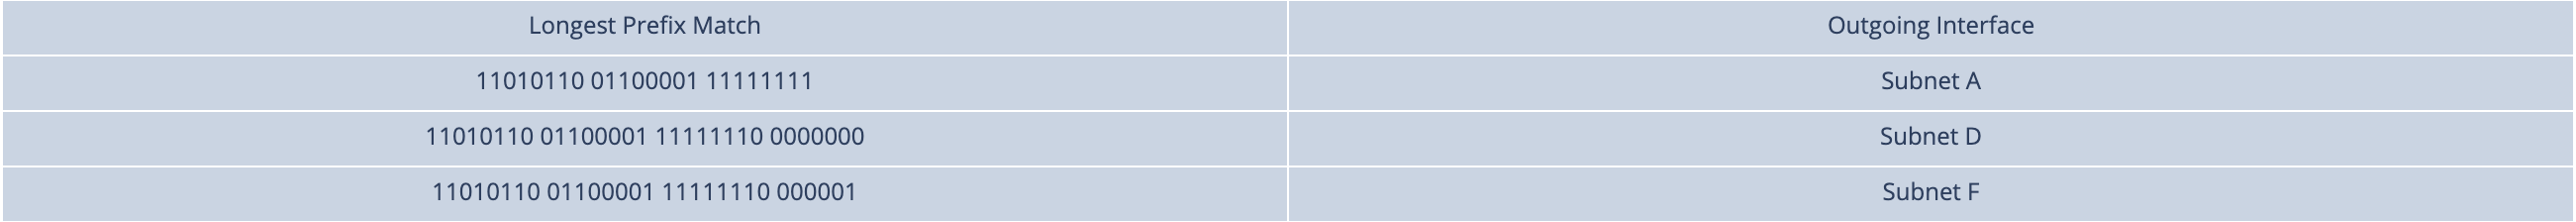
\includegraphics[width=1.0\columnwidth]{p12-1.png}
    \end{center}
    
    \begin{center}
        \textbf{Router 2}
        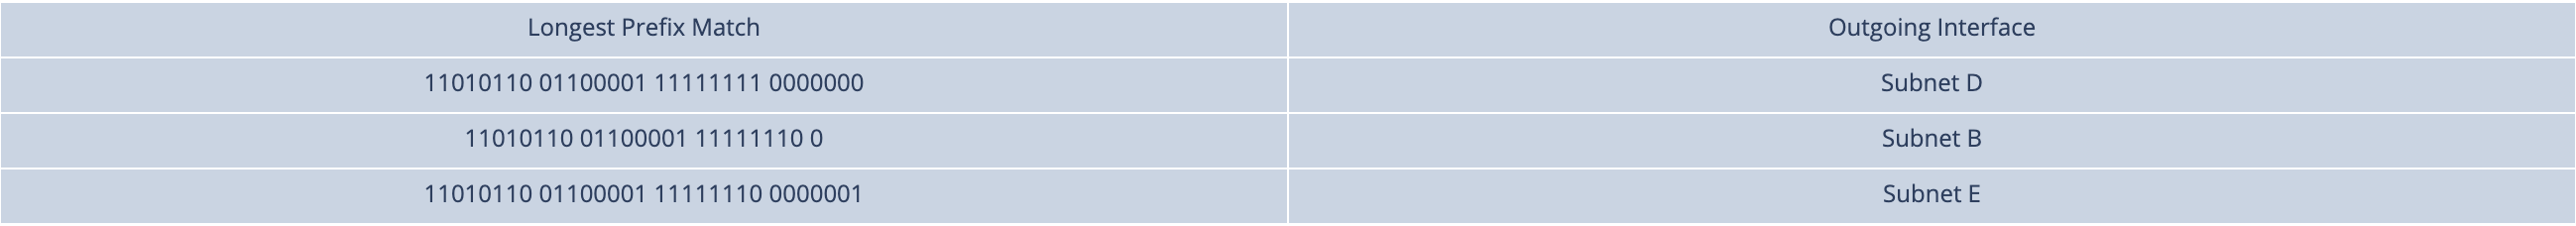
\includegraphics[width=1.0\columnwidth]{p12-2.png}
    \end{center}
    
    \begin{center}
        \textbf{Router 3}
        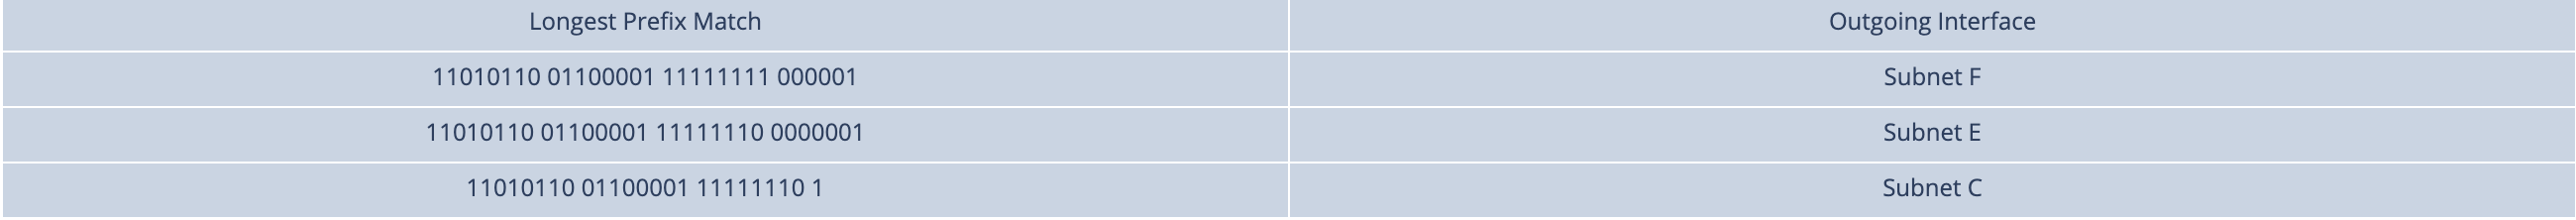
\includegraphics[width=1.0\columnwidth]{p12-3.png}
    \end{center}
}
\end{homeworkSection}
\end{homeworkProblem}
%----------------------------------------------------------------------------------------
\pagebreak


\begin{homeworkProblem}[P14]
\begin{homeworkSection}{}
\problemAnswer{
    Max size of data field of each fragment = 680 (IP header size: 20 bytes) \\
    Required Fragments = $\frac{2400 - 20}{680} = 4$ \\
    For each fragment, identification number would be 422 and except the last fragment it's size would be 700 bytes with flag = 1. Size of last fragment would be 360 bytes with flag = 0. The offsets of the fragments are 0, 85, 170, 255.
}
\end{homeworkSection}
\end{homeworkProblem}
%----------------------------------------------------------------------------------------
\pagebreak


\begin{homeworkProblem}[P18]
\begin{homeworkSection}{}
\problemAnswer{
    Not possible under NAT since p2p users are behind NAT and cannot make a TCP connection as it would drop the SYN packets arriving from WAN side.
}
\end{homeworkSection}
\end{homeworkProblem}
%----------------------------------------------------------------------------------------
\pagebreak

\begin{homeworkProblem}[Problem A]
\begin{homeworkSection}{a}
C4.5E.13.87 \\
\problemAnswer{
    B (20 bits)
}
\end{homeworkSection}


\begin{homeworkSection}{b}
C4.5E.22.09 \\
\problemAnswer{
    A (12 bits)
}
\end{homeworkSection}

\begin{homeworkSection}{c}
C3.41.80.02 \\
\problemAnswer{
    E (1 bit)
}
\end{homeworkSection}

\begin{homeworkSection}{d}
5E.43.91.12 \\
\problemAnswer{
    F (2 bits)
}
\end{homeworkSection}

\begin{homeworkSection}{e}
C4.6D.31.2E \\
\problemAnswer{
    C (12 bits)
}
\end{homeworkSection}

\begin{homeworkSection}{f}
C4.6B.31.2E \\
\problemAnswer{
    D (14 bits)
}
\end{homeworkSection}
\end{homeworkProblem}
%----------------------------------------------------------------------------------------
\pagebreak

\begin{homeworkProblem}[Problem B]
\begin{homeworkSection}{}
\problemAnswer{
    \textbf{Shared-memory router: } In case of multiple line cards, throughput can be limited by bus or by memory. Since bus rate is 200 Mhz and bus width is 32 bits, the bit rate is 200 * 32 = 6.4 Gbps. As the packets are put on bus for one way to memory and second time for output line card, the packet throughput by the bus is 3.2Gbps. To read and write 32-bit, it take 10ns. So the memory throughput is $\frac{32}{10^{-8}} = 3.2Gbps$. Therefore in this architecture both memory and bus are bottleneck\\
    
    \textbf{Bus Backplane Design: } In case multiple line cards, the bus is the bottleneck for throughput. Since each packet goes onto bus once i.e from input line card to output line card. Throughput of this architecture is 6.4Gbps \\
    
    \textbf{Switched Backplane Design: } Assuming that switched backplane is cross bar and puts no limitation on router's throughput. In case of $N$ line cards, the throughput is limited my memory at $\frac{32}{10^{-8}} = 3.2Gbps$. But due to head-of-line blocking, the actual throughput at each line card is 25\% of the memory i.e $3.2 * 0.25 = 0.8Gbps$. Therefore the router throughput is $N * 0.8Gbps$ \\
}
\end{homeworkSection}
\end{homeworkProblem}
%----------------------------------------------------------------------------------------
\pagebreak
\bibliographystyle{plain}
\bibliography{references} % see references.bib for bibliography management
\end{document}
%----------------------------------------------------------------------------------------
%	DONE
%----------------------------------------------------------------------------------------
